\section{Methodology} \label{sect:methodology}

\subsection{Framework Overview}
The core objective of our P4P framework, is to provide a proactive, lightweight, and multi-layer defense against poisoning attacks in FL. 
Existing defense strategies either rely on static aggregation rules or complex cryptographic primitives. 
Static rules (e.g., Krum, Trimmed Mean) treat client updates independently at each round and are vulnerable to collusion or stealthy poisoning, while cryptographic approaches (e.g., secure multiparty computation or blockchain-based logging) incur prohibitive overhead and still do not directly address model update manipulation. 
To overcome these limitations, we design P4P with three guiding principles: 


Proactivity: Instead of passively observing updates, the server actively queries clients using probe vectors derived from the global trajectory. 

Temporal awareness: Malicious behaviors often manifest gradually or intermittently. By chaining probe vectors across rounds, the server leverages historical consistency to expose stealthy strategies.

Lightweight robustness: Defense mechanisms must be practical in large-scale deployments. P4P transforms high-dimensional updates into low-dimensional probe responses, enabling efficient anomaly detection with minimal cost.


Figure~\ref{fig:framework} illustrates the overall architecture of P4P. At each round, the server constructs a probe vector, broadcasts it to clients, collects probe responses and updates, applies multi-layer detection, and finally aggregates only trusted contributions into the global model. 

\subsection{Probe Vector Construction}

One of the central novelties of P4P lies in the construction and use of \textit{probe vectors}. 
Rather than assuming that the majority of client updates are benign, which may not hold under collusion, the server instead relies on its own historical trajectory as a stable reference. 

Given the global parameters $W_t \in \mathbb{R}^d$ at round $t$, the probe vector is defined as:

\begin{equation}
    v_t = W_t - W_{t-1}.
\end{equation}

This formulation captures the \textit{incremental direction} of model evolution between two consecutive rounds. 
It has two desirable properties: (1) it encodes temporal history, meaning that adversaries cannot easily alter it without consistently corrupting many rounds; (2) it is model-dependent but data-agnostic, requiring no access to raw data or trusted clean datasets. 

Alternative approaches, such as computing references from small server-side datasets, are either unrealistic (clean data may not exist) or introduce bias (server data not representative of client distributions). 
By contrast, the probe vector leverages only information already available to the server.

As shown in Figure \ref{fig:pipeline}, the probe vector provides a global reference that reduces Non-IID bias. While benign clients align with the probe, suspicious clients deviate due to Non-IID heterogeneity, and malicious clients cluster in the opposite direction, enabling clustering-based separation.

\begin{figure}[ht]
  \centering
  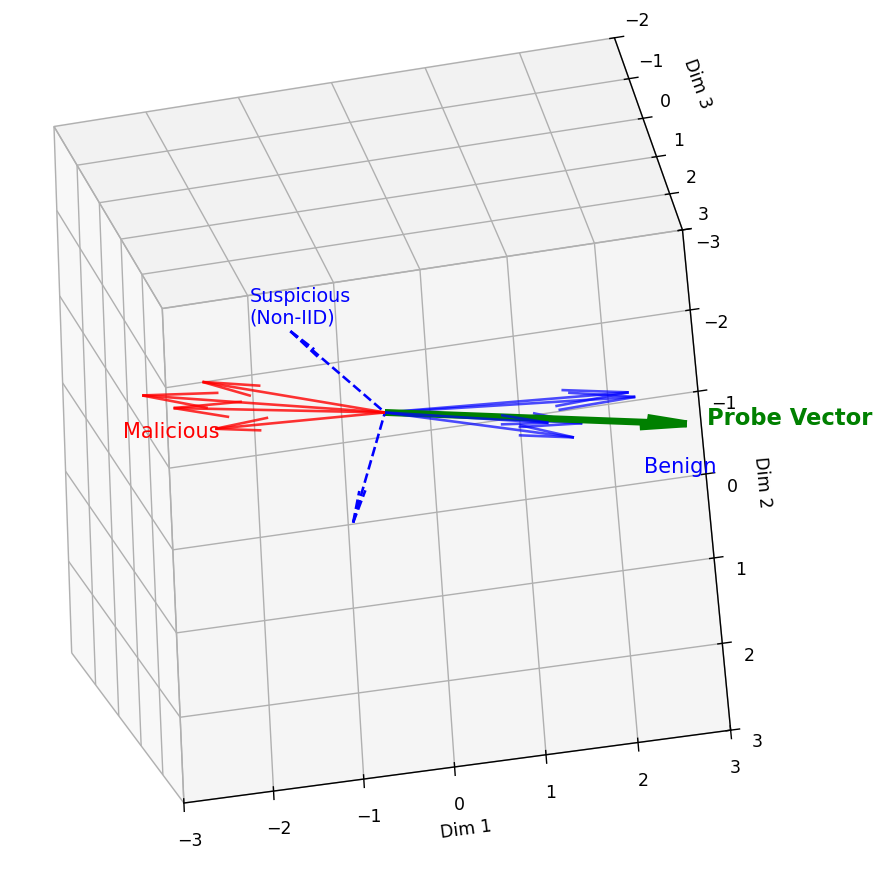
\includegraphics[width=1\linewidth]{Screenshot 2025-09-30 145946.png}
  \caption{Caculate consines similarity between Clients and Probe Vector then Clustering}
  \label{fig:pipeline}
\end{figure}

\subsection{Client Probe Response}

Upon receiving $v_t$, each client $C_i$ computes its \textit{probe response} $r_i^t$ by measuring the cosine similarity between its local update $\Delta W_i^t$ and $v_t$:

\begin{equation}
    r_i^t = \frac{\langle \Delta W_i^t, v_t \rangle}{\|\Delta W_i^t\|_2 \cdot \|v_t\|_2}.
\end{equation}

This scalar response compresses high-dimensional updates into a single interpretable score. 
High values ($r_i^t \approx 1$) indicate alignment with the global trajectory, as expected from benign clients. 
Low or negative values indicate divergence or sign flipping, typical of malicious updates. 

This transformation is crucial for scalability: a model with millions of parameters can be reduced to a one-dimensional similarity measure per client, enabling lightweight clustering and anomaly detection. 
Moreover, since all clients are evaluated against the same reference $v_t$, non-IID heterogeneity is normalized, reducing false positives.

\subsection{Multi-layer Defense Mechanism}
To ensure robustness, P4P does not rely solely on probe responses but integrates them into a multi-layer pipeline.

\subsubsection{L2-norm Filtering}
\begin{figure}[ht]
  \centering
  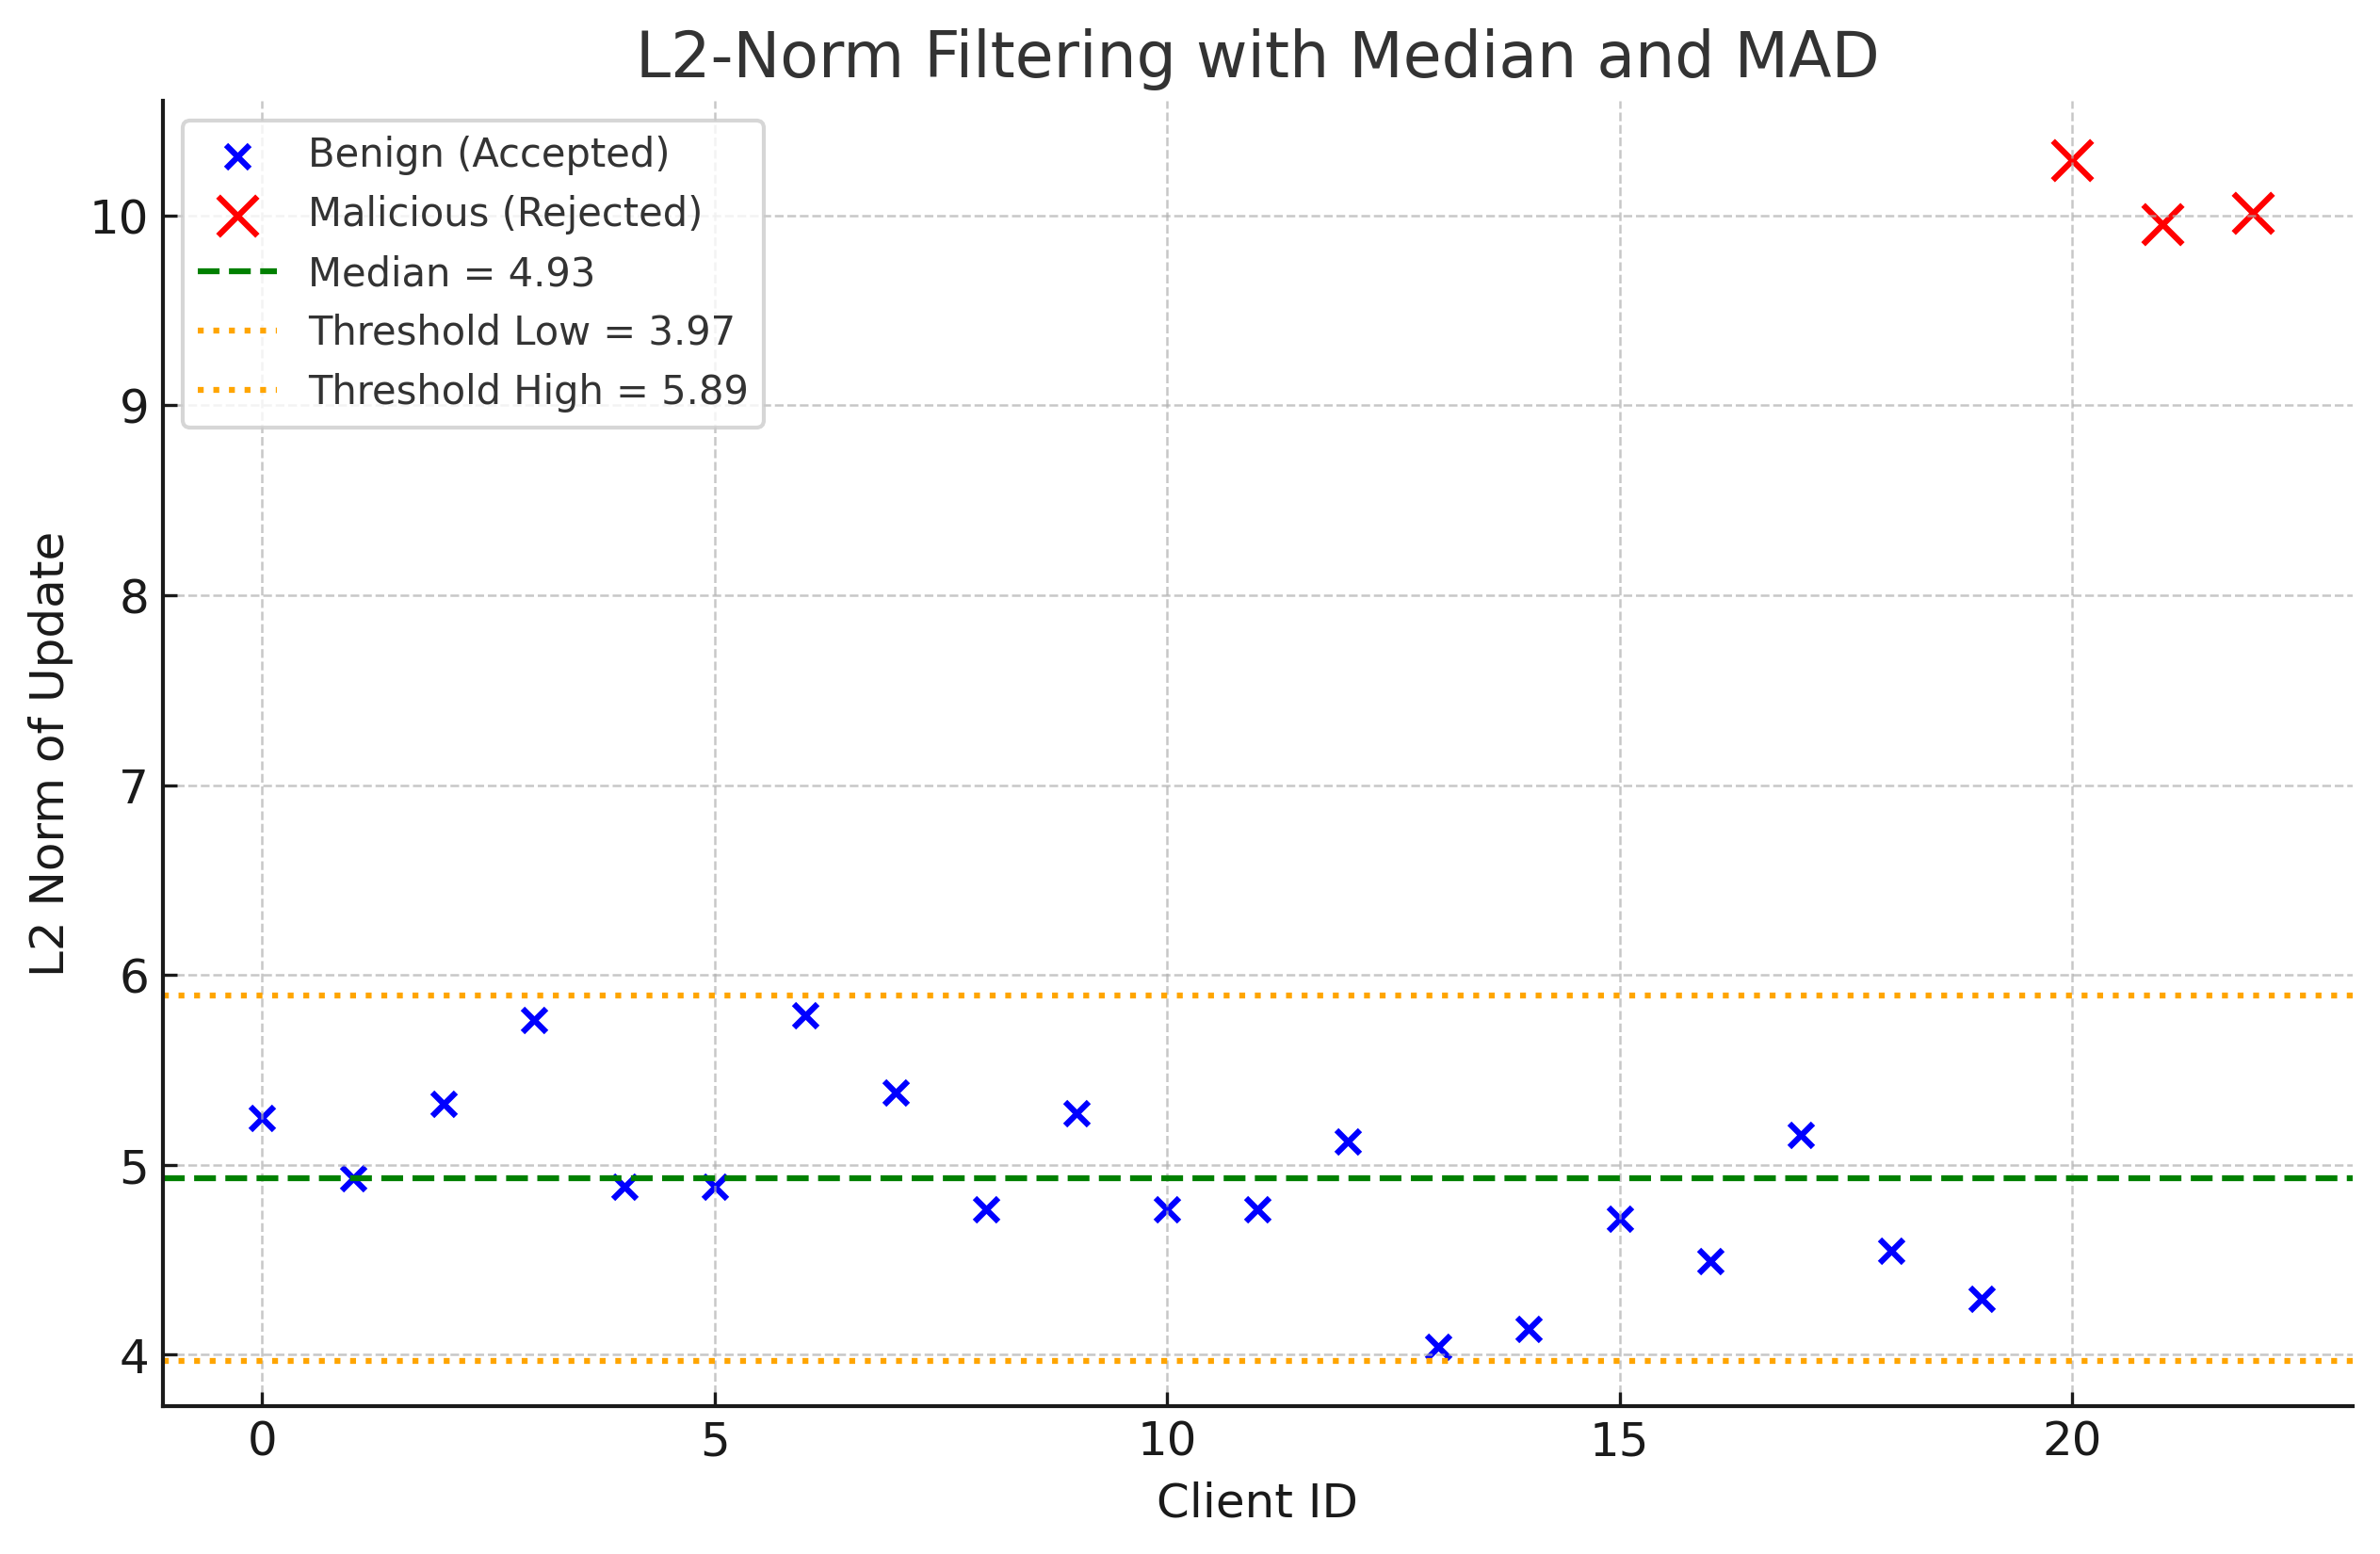
\includegraphics[width=1\linewidth]{l2_norm_filtering.png}
  \caption{Graph construction and representation process of heterogeneous graphs.}
  \label{fig:MADFilter}
\end{figure}
We first evaluate the scale of each update by its L2 norm:

\begin{equation}
    \|\Delta W_i^t\|_2 = \sqrt{\sum_{j=1}^d (\Delta W_{i,j}^t)^2}.
\end{equation}

Malicious clients often inject updates with abnormally large magnitudes to dominate aggregation. 

To robustly filter such outliers, we apply Median Absolute Deviation (MAD):

\begin{equation}
    \text{MAD} = \text{median} \left( \big| \|\Delta W_i^t\|_2 - \text{median}(\|\Delta W^t\|_2) \big| \right).
\end{equation}

Updates exceeding a threshold (e.g., $3 \times$ MAD) are temporarily flagged. 

This step prevents simple scaling attacks. As show in Figure~\ref{fig:MADFilter}, this step prevents attacks base on scaling weight.


\subsubsection{Probe-based Anomaly Detection}
Next, the probe responses $\{r_i^t\}$ are analyzed using an ensemble of detectors:

\begin{itemize}
    \item \textbf{KMeans clustering}: partitions responses into two groups; minority clusters are suspect.
    \item \textbf{DBSCAN}: detects density-based anomalies; isolated clients (label $=-1$) are suspect.
    \item \textbf{Isolation Forest}: identifies statistical outliers; responses with low isolation scores are suspect.
\end{itemize}

% =============================
% Algorithm 2: Probe-based Anomaly Detection
% =============================
\begin{algorithm}[H]
\caption{Probe-based Anomaly Detection (Ensemble Voting)}
\KwIn{Probe responses $\{r_i^t\}_{i=1}^N$, client IDs $\{C_i\}$}
\KwOut{Suspicious client set $\mathcal{S}_{anom}$}

Initialize votes[$i$] $\gets 0$ for all clients\;

\textbf{Step 1: KMeans Clustering}\;
Cluster $\{r_i^t\}$ into 2 groups\;
Assign vote[$i$]++ if client $i$ belongs to minority cluster\;

\textbf{Step 2: DBSCAN}\;
Run DBSCAN on $\{r_i^t\}$\;
Assign vote[$i$]++ if client $i$ is labeled as noise ($-1$)\;

\textbf{Step 3: Isolation Forest}\;
Fit Isolation Forest on $\{r_i^t\}$\;
Assign vote[$i$]++ if client $i$ is predicted as outlier\;

$\mathcal{S}_{anom} \gets \{ i \mid \text{votes}[i] \geq 2 \}$\;

\Return $\mathcal{S}_{anom}$\;
\end{algorithm}
Each detector provides a vote, and a client is considered suspicious if flagged by at least two. 
This ensemble approach increases robustness against adaptive attacks designed to bypass a single detector.



\subsubsection{Temporal Suspicion Scoring}
To address intermittent poisoning and reduce false positives, we introduce a suspicion score $s_i^t$:

\begin{equation}
    s_i^t = \max(0, s_i^{t-1} + \delta_i^t - \gamma),
\end{equation}

where $\delta_i^t=1$ if client $C_i$ is flagged at round $t$ and $0$ otherwise, and $\gamma$ is a decay factor allowing benign clients to recover over time. 
If $s_i^t > \theta$, the client is permanently removed. 
% =============================
% Algorithm 3: Temporal Suspicion Scoring
% =============================
\begin{algorithm}[H]
\caption{Temporal Suspicion Scoring}
\KwIn{Previous scores $s_i^{t-1}$, suspicious set $\mathcal{S}_{anom}$, decay $\gamma$, threshold $\theta$}
\KwOut{Updated scores $s_i^t$, permanently removed clients $\mathcal{R}$}

$\mathcal{R} \gets \emptyset$\;

\ForEach{client $i$}{
    \eIf{$i \in \mathcal{S}_{anom}$}{
        $s_i^t \gets s_i^{t-1} + 1$\;
    }{
        $s_i^t \gets \max(0, s_i^{t-1} - \gamma)$\;
    }
    \If{$s_i^t > \theta$}{
        add $i$ to $\mathcal{R}$\;
    }
}
\Return $(s_i^t, \mathcal{R})$\;
\end{algorithm}

This mechanism leverages temporal history, ensuring that malicious behavior accumulating over rounds is detected, while benign clients with occasional deviations are not unfairly penalized.
% ===================================
% Algorithm 3: Server-side Detection + Aggregation
% ===================================
\begin{algorithm}[H]
\caption{ServerProcedure($W_t, \{\Delta W_i^t, r_i^t\}, \{s_i\}$)}
\KwIn{Global model $W_t$, client updates $\{\Delta W_i^t\}$, probe responses $\{r_i^t\}$, suspicion scores $\{s_i\}$}
\KwOut{Updated global model $W_{t+1}$}

\tcp{L2-norm filtering}
Compute $l_i = \|\Delta W_i^t\|_2$\;
$m \gets \text{median}(\{l_i\})$, \quad $\text{MAD} \gets \text{median}(|l_i - m|)$\;
$\mathcal{S}_{norm} \gets \{ i : |l_i - m| \leq \tau \cdot \text{MAD} \}$\;

\tcp{Probe-based ensemble anomaly detection}
Initialize votes[$i$] $\gets 0$\;
Run KMeans, DBSCAN, Isolation Forest on $\{r_i^t\}$\;
Increment votes[$i$] for outliers\;
$\mathcal{S}_{anom} \gets \{ i : \text{votes}[i] \geq 2 \}$\;

\tcp{Temporal suspicion scoring}
\ForEach{$i \in \mathcal{S}_{norm}$}{
    \eIf{$i \in \mathcal{S}_{anom}$}{
        $s_i \gets s_i + \delta$\;
    }{
        $s_i \gets \max(0, s_i - \gamma)$\;
    }
    \If{$s_i > \theta$}{
        mark client $i$ as permanently malicious\;
    }
}

\tcp{Aggregation from trusted clients}
$\mathcal{S}_{trust} \gets \mathcal{S}_{norm} \setminus \mathcal{R}$\;
$W_{t+1} \gets W_t + \eta \cdot \frac{\sum_{i \in \mathcal{S}_{trust}} \Delta W_i^t}{|\mathcal{S}_{trust}|}$\;

\Return $W_{t+1}$\;
\end{algorithm}
\subsection{Robust Aggregation}
Finally, trusted updates are aggregated to update the global model. 
We adopt a weighted FedAvg scheme:

\begin{equation}
    W_{t+1} = W_t + \eta \cdot \frac{\sum_{i=1}^N \omega_i^t \Delta W_i^t}{\sum_{i=1}^N \omega_i^t},
\end{equation}

where $\omega_i^t \in \{0,1\}$ indicates whether client $C_i$ is trusted at round $t$, and $\eta$ is the global learning rate. 
\usepackage[ruled,vlined]{algorithm2e}



By integrating multiple layers of defense before aggregation, P4P minimizes the influence of malicious updates and maintains the integrity of the global model.

\subsection{Workflow Summary}
The complete P4P workflow can be summarized as follows:

\begin{enumerate}
    \item \textbf{Probe vector construction:} The server computes $v_t = W_t - W_{t-1}$ from consecutive global models.
    \item \textbf{Client probing:} Each client computes $r_i^t$ by measuring cosine similarity between $\Delta W_i^t$ and $v_t$, and returns both $\Delta W_i^t$ and $r_i^t$.
    \item \textbf{Multi-layer detection:} The server applies L2-norm filtering, ensemble anomaly detection on $\{r_i^t\}$, and temporal suspicion scoring.
    \item \textbf{Robust aggregation:} Updates from trusted clients are aggregated to form $W_{t+1}$.
\end{enumerate}